\section{Behaviour}
\label{Behaviour}
\subsection{Strategy}
The overall strategy for this year was to attempt to kick the ball towards the opponents goal as quickly and as often as possible. To do this the general behaviour was to walk to the kicking position where the opponents goal was lined up and then kick. Since we only kicked forward this was a calculated position based on the position of the ball on the field. In terms of team behaviour, we attmepted to always have one robot chasing the ball while any other robots tried to move into their ideal position. In an attempt to simplify the writing of behaviour code the walk engine included many planning functions so that behaviours simply pass the walk engine the desired relative position and heading and the walk engine will take it there. These path planning paths were built around the desired behaviours so many complex decisions were not required. To carry out this overall strategy a number of sub-behaviours were developed. These were run depending on current circumstances as shown in ~\autoref{fig:PlayerTaskDecision}.

\begin{figure}[!h]
\begin{center}
   \leavevmode
    \scalebox{0.8} {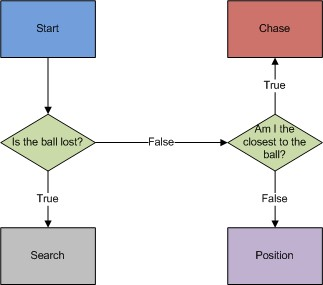
\includegraphics{figs/FieldPlayerTaskDecision.jpg} }
    \caption{Player task decision tree}
    \label{fig:PlayerTaskDecision}
\end{center}
\end{figure}



\subsection{Searching}
The trigger for searching was greatly improved upon from last year. Previously the robot would search if it could simply not see the ball. Howevever when moving into position we found that it may be advantageous to lose sight of the ball for short amounts of time to gain an increase in walking speed. Because of this some high level properties were created 'isBallLost' and 'amILost'. The isBallLost property takes into account the number of vision frames since the ball was last seen as well as the current world model uncertainty to determine if yourself or the team as a whole has lost the ball. Because the world model ball also includes information from team mates if they are providing the robot with good estimates of the ball position it may not be required to search. Likewise if the worldmodel uncertainties indicate that the predictions are accurate searching again may not be required. The amILost property was used to determine the validity of the robots world model estimates. Once the uncertainty reached a predefined threshold the robot would attempt to localise by doing a pan at a level likely to see the goal posts and field lines.\\

Once we had determined that a ball was lost and must be found we used a simple searching method. The robot would pan its head vertically from top to bottom while turning in a circle. The horizontal angle of the camera was set to one step worth of a turn towards the turning direction so that if a ball is seen at the completion of the next turn step it can begin moving forwards towards it. We would alternate cameras for each turn starting with the camera we deemed most likely to see the ball based on its estimated distance. However this sometimes proved frustrating since it would sometimes choose the wrong camera and would then require more than a complete turn to find the ball.\\

The chasing behaviour is the main part of our gameplay. It involves walking to an ideal kicking position. turning to line up the goal, then lining up the ball and finally kicking. To simplify the writing of behaviours we created another high level property 'isOpponentsGoalLinedUp'. This is determined very simply, if the left hand post of the opponents goal is on our left and the right hand post is on our right then the goal is lined up for a kick. There were a number of states in the chasing behaviour. The transition conditions between states cand be found in \autoref{fig:ChasingStateDiagram}.
\begin{enumerate}
\item \textbf{Approach} The robot will move towards the desired kicking position. This is situated on the opposited side of the ball to the opponents goal.
\item \textbf{Position} The robot will turn to face the opponents goal, lining it up so that it is facing between the two posts.
\item \textbf{Kick} The robot will line one of its feet up to the ball. One the ball is within the effective kicking range the kick sequence will be called.
\end{enumerate}

\subsection{Chasing}
\begin{figure}[!h]
\begin{center}
   \leavevmode
    \scalebox{0.8} {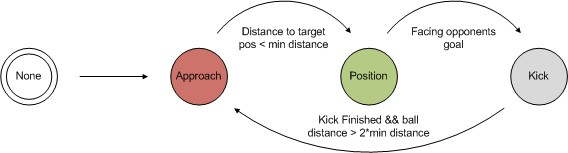
\includegraphics{figs/FieldPlayerChasingStates.jpg} }
    \caption{Chasing behaviour state diagram}
    \label{fig:ChasingStateDiagram}
\end{center}
\end{figure}

\subsection{Positioning}
The positioning behaviour simply moves to a fixed point on the field. Once close to the desired field position the robot turns to face the ball. If the ball can be seen the robot will track the ball. If not the robot will face towards the estimated ball position and pan to look for the ball and view localisation landmarks.
